\documentclass[12pt]{article}
\usepackage[paperwidth=188.88mm,paperheight=246mm,textwidth=427.64493pt,textheight=596.5pt,centering]{geometry}
\usepackage{graphicx}
\usepackage{subcaption}
\usepackage[T1]{fontenc}
\captionsetup{font=small}
\begin{document}
\begin{figure}[t]
\centering
\begin{subfigure}[t]{.49\linewidth}
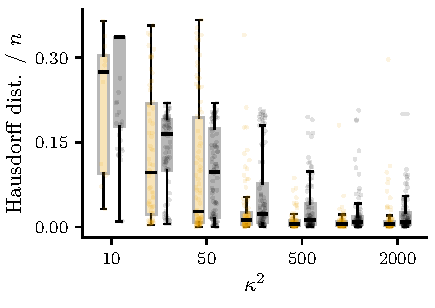
\includegraphics[width=\linewidth]{M3/M3_delta3_haus_box.pdf}
\caption{Location error.}
\end{subfigure}\hfill
\begin{subfigure}[t]{.49\linewidth}
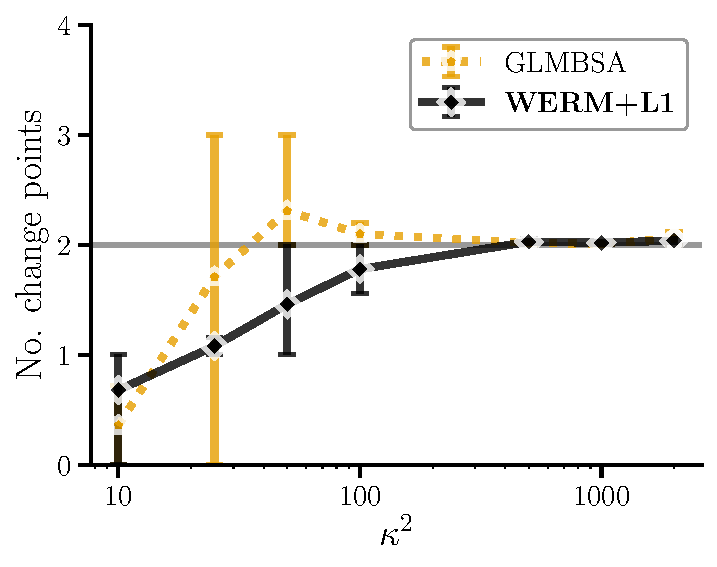
\includegraphics[width=\linewidth]{M3/M3_delta3_size_line.pdf}
\caption{Selected counts.}
\end{subfigure}
\caption{M3, $\delta=3$, $\alpha=0.1$: saved 100-trial comparison.
Boxplots show the median and interquartile range with 1.5-IQR whiskers
and faint trial points. Count lines show means with the canonical
absolute distances to the first and third quartiles.}
\end{figure}
\begin{figure}[h]
\centering
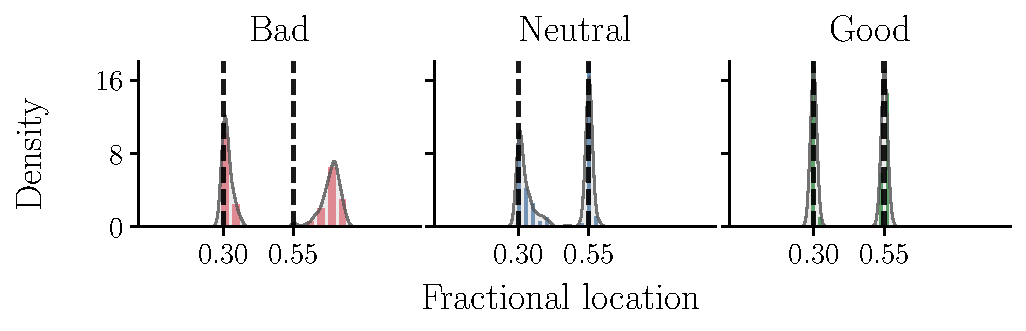
\includegraphics[width=\linewidth]{E_PRIOR/prior_estimated_locations.pdf}
\caption{Estimated locations under bad, neutral and good priors.
The canonical histogram display uses 12 bins and a Gaussian KDE;
dashed lines mark truth. Density peaks above 18 are clipped.}
\end{figure}
\begin{figure}[h]
\centering
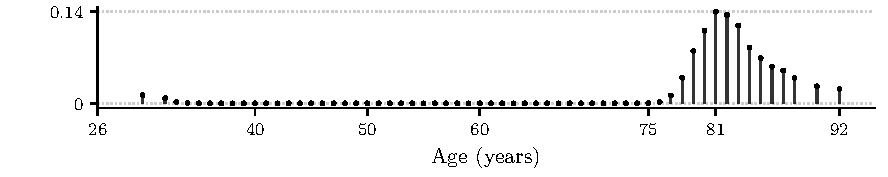
\includegraphics[width=\linewidth]{Myocardial/rank3_conditional_posterior.pdf}
\caption{Case A myocardial posterior conditional on one change point.}
\end{figure}
\end{document}
